% generated by experiments/dynarapid/make_tex.py - do not edit
\begin{figure}[t]
\centering
\definecolor{rwc1}{HTML}{2a78d6}
\definecolor{rwc2}{HTML}{eb6834}
\definecolor{rwc3}{HTML}{1baf7a}
\definecolor{rwc4}{HTML}{eda100}
\definecolor{rwc5}{HTML}{e87ba4}
\definecolor{rwc6}{HTML}{008300}
\definecolor{rwink}{HTML}{52514e}
\definecolor{rwgrid}{HTML}{e6e5e1}
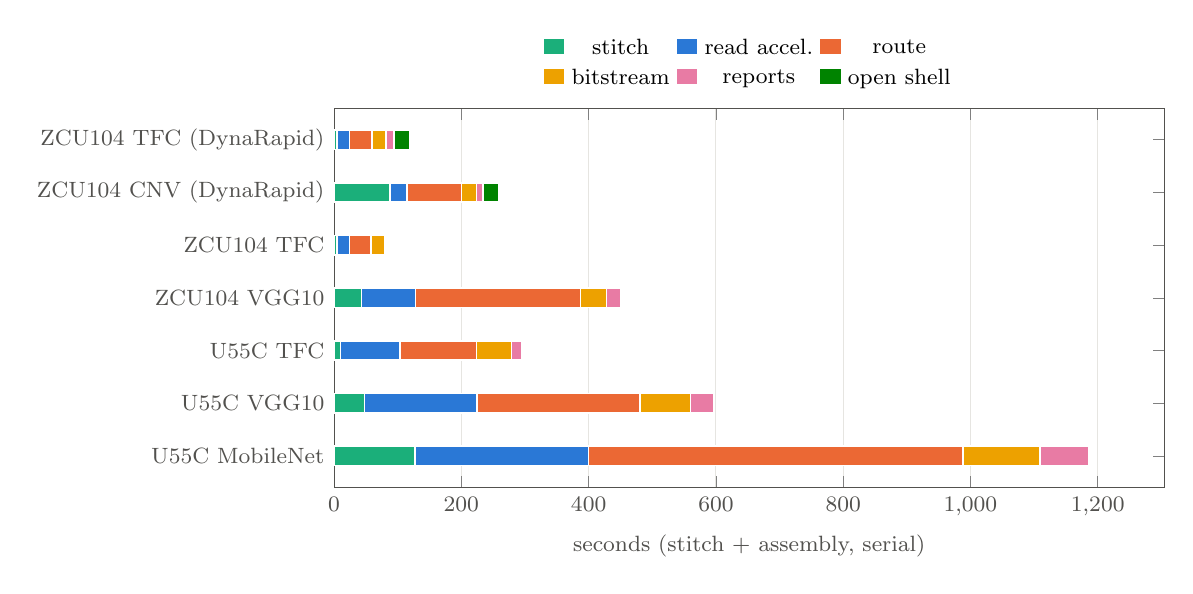
\begin{tikzpicture}
\begin{axis}[
  xbar stacked, bar width=7pt, width=\columnwidth, height=6.4cm,
  symbolic y coords={a0,a1,a2,a3,a4,a5,a6}, ytick=data, yticklabels={{ZCU104 TFC (DynaRapid)},{ZCU104 CNV (DynaRapid)},{ZCU104 TFC},{ZCU104 VGG10},{U55C TFC},{U55C VGG10},{U55C MobileNet}}, y dir=reverse,
  yticklabel style={font=\footnotesize, align=right, rwink},
  xlabel={seconds (stitch + assembly, serial)}, xmin=0,
  xmajorgrids, grid style={rwgrid}, axis line style={rwink}, tick label style={font=\footnotesize, rwink},
  label style={font=\footnotesize, rwink},
  legend style={font=\footnotesize, draw=none, fill=none, at={(0.5,1.02)}, anchor=south, legend columns=3},
  reverse legend=false,
]
\addplot[fill=rwc3, draw=white, line width=0.6pt] coordinates {(5,a0) (88,a1) (5,a2) (43,a3) (10,a4) (48,a5) (127,a6)};
\addlegendentry{stitch}
\addplot[fill=rwc1, draw=white, line width=0.6pt] coordinates {(19,a0) (27,a1) (19,a2) (85,a3) (94,a4) (177,a5) (273,a6)};
\addlegendentry{read accel.}
\addplot[fill=rwc2, draw=white, line width=0.6pt] coordinates {(36,a0) (85,a1) (34,a2) (259,a3) (120,a4) (256,a5) (588,a6)};
\addlegendentry{route}
\addplot[fill=rwc4, draw=white, line width=0.6pt] coordinates {(22,a0) (24,a1) (21,a2) (41,a3) (55,a4) (79,a5) (121,a6)};
\addlegendentry{bitstream}
\addplot[fill=rwc5, draw=white, line width=0.6pt] coordinates {(12,a0) (10,a1) (2,a2) (22,a3) (16,a4) (37,a5) (77,a6)};
\addlegendentry{reports}
\addplot[fill=rwc6, draw=white, line width=0.6pt] coordinates {(25,a0) (25,a1) (0,a2) (0,a3) (0,a4) (0,a5) (0,a6)};
\addlegendentry{open shell}
\end{axis}
\end{tikzpicture}
\caption{The serial tail on the ZCU104 and the U55C. The island flow overlaps opening the shell with the
island P\&R; the DynaRapid assembly opened it afterwards.}
\label{fig:assembly}
\end{figure}
